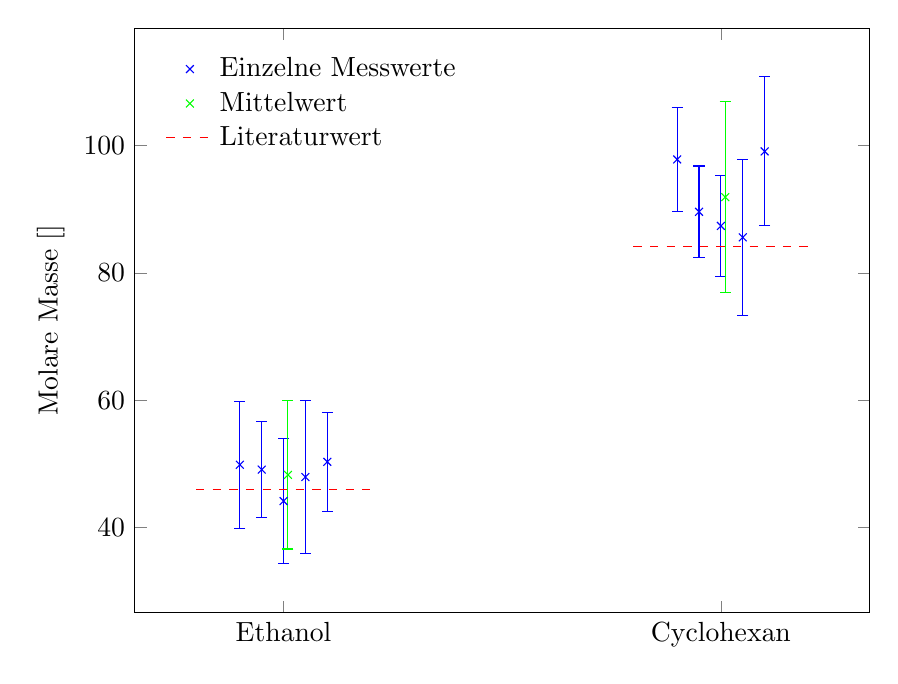
\begin{tikzpicture}
\begin{axis}[width = .9\textwidth, height = 9cm,
	xtick={.3,1.3},
	xticklabels={Ethanol, Cyclohexan},
	ylabel = {Molare Masse [\si{\g\per\mol}]},
	legend style={draw=none, legend cell align = left}, legend pos = north west]

\addplot[blue, only marks, error bars/y dir = both, error bars/y explicit, mark = x] table[x=x,y=y, y error = err] {
x	y	err
.2	49.8785358849	9.9841273896
.25	49.1228004927	7.5637826811
.3	44.1837424177	9.8251242482
.35	47.9601306586	11.9992384215
.4	50.343242741	7.7520048157
};

\addplot[green, only marks, error bars/y dir = both, error bars/y explicit, mark = x] table[x=x,y=y, y error = err] {
x	y	err
.31	48.297690439	11.634048942
};

\addplot[dashed, red, domain=.1:.5] {46.07};

\legend{Einzelne Messwerte, Mittelwert, Literaturwert}

\addplot[blue, only marks, error bars/y dir = both, error bars/y explicit, mark = x] table[x=x,y=y, y error = err] {
x	y	err
1.2	97.8010507547	8.1771956813
1.25	89.5807038163	7.1869095787
1.3	87.3668622188	7.9636160815
1.35	85.5759194104	12.2549480494
1.4	99.0578399583	11.6920686252
};

\addplot[green, only marks, error bars/y dir = both, error bars/y explicit, mark = x] table[x=x,y=y, y error = err] {
x	y	err
1.31	91.8764752317	14.9681458409
};
\addplot[dashed, red, domain=1.1:1.5] {84.16};
\end{axis}
\end{tikzpicture}